\documentclass[12pt]{beamer}

\usetheme{metropolis}
\usepackage{appendixnumberbeamer}

% Notes for pdfpc
\usepackage{pdfpc}

\usepackage{booktabs}
\usepackage[scale=2]{ccicons}

\usepackage{pgfplots}
\usepgfplotslibrary{dateplot}

\usepackage{listings}
\usepackage{listingsutf8}

% colored bulletpoints (https://tex.stackexchange.com/questions/329990/how-do-i-change-the-color-of-itemize-bullet-specific-and-default)
\usepackage{enumitem,xcolor}

\usepackage[backend=biber,
            style=alphabetic,
            minalphanames=3, maxalphanames=4,
            maxbibnames=20]{biblatex} % to generate the bibliography
\addbibresource{library.bib}           % name of the bib-file

%\useinnertheme[shadow]{rounded}

\usepackage{xspace}
\newcommand{\themename}{\textbf{\textsc{metropolis}}\xspace}

% src: https://github.com/marekaf/docker-lstlisting/blob/master/latex.tex
\lstdefinelanguage{docker}{
  keywords={FROM, RUN, COPY, ADD, ENTRYPOINT, CMD,  ENV, ARG, WORKDIR, EXPOSE, LABEL, USER, VOLUME, STOPSIGNAL, ONBUILD, MAINTAINER, del, upgrade},
  keywordstyle=\color{blue}\bfseries,
  identifierstyle=\color{black},
  sensitive=false,
  comment=[l]{\#},
  commentstyle=\color{purple}\ttfamily,
  stringstyle=\color{red}\ttfamily,
  morestring=[b]',
  morestring=[b]"
}
\lstset{basicstyle=\ttfamily,
  showstringspaces=false,
  commentstyle=\color{red},
  keywordstyle=\color{blue},
  inputencoding=utf8,
  extendedchars=true
}

% https://tex.stackexchange.com/questions/224093/adding-keywords-to-existing-language-for-listings-package
\lstdefinelanguage{OwnBash}{%
  language     = bash,
  morekeywords = {docker, \$docker},
  literate = {-}{-}1, % <------ trick! https://tex.stackexchange.com/questions/282263/lstlisting-keep-hyphens-dashes-from-combining-into-one
}

%%% Frameheader with Image
\makeatletter
\setbeamertemplate{frametitle}{%
    \nointerlineskip%
    \begin{beamercolorbox}[%
        wd=\paperwidth,%
        sep=0pt,%
        leftskip=\metropolis@frametitle@padding,%
        rightskip=\metropolis@frametitle@padding,%
    ]{frametitle}%
    \metropolis@frametitlestrut@start%
    \insertframetitle%
    \nolinebreak%
    \metropolis@frametitlestrut@end%
    \hfill
    \raisebox{-1.2ex}{
        \includegraphics[height=4ex,keepaspectratio]{images/logos/losfuzzys_logo.png}
    }
  \end{beamercolorbox}%
}
\makeatother

%%% Titlepage with LOGO
\titlegraphic{%
  \hfill
  \includegraphics[width=6cm,height=1.6cm,keepaspectratio]{images/logos/losfuzzys_logo.png}
  \hfill

}


\title{Introduction to Docker}
\subtitle{What it is and how to use it}
\date{\today}
\author{LosFuzzys}
% \institute{TU}
% \titlegraphic{\hfill\includegraphics[height=1.5cm]{logo.pdf}}

\begin{document}

\maketitle

% \begin{frame}{Table of contents}
%   \setbeamertemplate{section in toc}[sections numbered]
%   \tableofcontents[hideallsubsections]
% \end{frame}

\begin{frame}[fragile]{What will be smaller: No one}
    We prepared some challenges for your. \\
    They can all be solved with commands presented here
    \begin{itemize}[label=\textcolor{black}{\textbullet}]
        \item Docker Runner 1
        \item Docker Runner 2
        \item Docker Inspector
        \item Docker Exposer
        \item Docker Copyer
    \end{itemize}
    The name gives a hint on what to do\\
    Also, \emph{Docker Exposer} used information obtained during \emph{Docker Inspector}
\end{frame}

\section{What is Docker?}

\begin{frame}{About Docker}
    Docker lets us distribute software in containers. \\
    These containers ship with the software and all their dependencies
    \begin{itemize}
        \item Easy deployment
        \item Reproducability (if used right)
        \item Dependencies between containers can be described easily
    \end{itemize}
\end{frame}

\begin{frame}{Docker vs. VM}
   \begin{figure}
        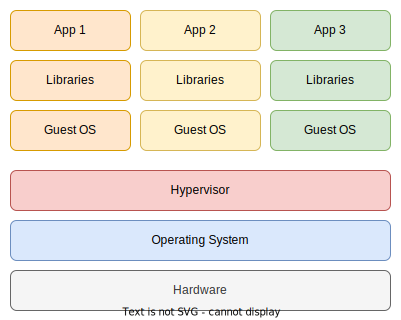
\includegraphics[width=.48\linewidth]{images/virtualisation_vs_container_vm.png}\hfill
        \pause
        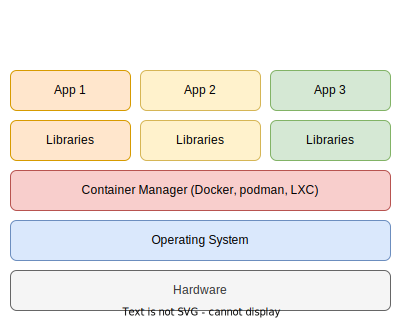
\includegraphics[width=.48\linewidth]{images/virtualisation_vs_container_docker.png}
    \end{figure} 
\end{frame}

\begin{frame}{Benefits and Drawbacks}
    \begin{itemize}[label=\textcolor{green}{\textbullet}]
        \item No guest OS is needed
        \item Container are ready as soon as they are spawned
        \item lightweight if build correctly
    \end{itemize}
    \begin{itemize}[label=\textcolor{red}{\textbullet}]
        \item Exploits in the Kernel can be exploited
        \item Access to the filesystem might be problematic
        \item Container needs to be build for the hosts OS
        \item \textcolor{red}{docker.socket}
    \end{itemize}
\end{frame}

\begin{frame}{What can run where}
    Linux container can only run on Linux machines. \\
    But why does Docker-Desktop (for Windows or MacOS) work? \\
    \begin{itemize}
        \item Under the hood they launch a Linux-vm and this VM runs the container \cite{Ferquel_2019}
    \end{itemize}
\end{frame}

\begin{frame}{Where do we use docker?}
    LosLuzzys uses docker (or containers) everywhere \\
    All our CTFs run on containers
    \begin{itemize}[label=\textcolor{black}{\textbullet}]
        \item fuzzy.land
        \item GlacierCTF
        \item KaindorfCTF
    \end{itemize}
    Also our internal services run in containers
\end{frame}


\begin{frame}{Dockerfile, Image and Container}
    There are three distinct components:
    \begin{itemize}
        \item Dockerfile: describes how the Dockerimage looks
        \item Dockerimage: blueprint for Container
        \item Dockercontainer: The thing that is running
    \end{itemize}

    \begin{figure}
        \centering
        \includegraphics[width=0.8\textwidth]{images/docker_file_image_container.png}
        % \includegraphics[width=0.6\textwidth]{images/relation_between_file_image_container.png}
    \end{figure}
\end{frame}

\section{Dockerimages}

\begin{frame}{What are images}
    The Images are the blueprints for the container\\
    They can be shared with others. \\
    \begin{itemize}
        \item Dockerhub \url{https://hub.docker.com/}
        \item Github Container Registry
    \end{itemize}
\end{frame}


\begin{frame}{Dockerhub}
    \only<1>{
        \begin{figure}
            \includegraphics[width=\linewidth]{images/dockerhub/dockerhub_python_search.png}\hfill
        \end{figure}
    }
    \only<2>{
        \begin{figure}
            \includegraphics[width=\linewidth]{images/dockerhub/dockerhub_python_page.png}\hfill
        \end{figure} 
    }
    \only<3>{
        \begin{figure}
            \includegraphics[width=\linewidth]{images/dockerhub/dockerhub_python_page_tags.png}\hfill
        \end{figure} 
    }
\end{frame}


\begin{frame}{Tags}
    Tags are a way to specify the version of a image.
    Example:
    \begin{itemize}
        \item python:3.10.13-bookworm
        \item python:3.9.18-alpine3.17
        \item httpd:2.4-alpine3.18
        \item postgresql:latest
    \end{itemize}
    Be careful, sometimes container break if the wrong image is used
\end{frame}

\begin{frame}[fragile]{Pulling, listing and deleting image}
    To pull an image
    \begin{lstlisting}[language=OwnBash]
$docker pull alpine:3.18
    \end{lstlisting}
    List all pulled image
    \begin{lstlisting}[language=OwnBash]
$docker image ls
    \end{lstlisting}
    Remove a previously pulled image
    \begin{lstlisting}[language=OwnBash]
$docker image rm alpine:3.18
    \end{lstlisting}
\end{frame}


\begin{frame}[fragile]{Start a container}
    General commandformat
    \begin{lstlisting}[language=OwnBash]
$docker run [OPTIONS] IMAGE[:TAG|@DIGEST] \
    [COMMAND] [ARG...]
    \end{lstlisting}
    The image gets pulled if it does not exist.\\
    Be careful, sometimes this is unwanted
    \begin{lstlisting}[language=OwnBash]
$docker run hello-world
    \end{lstlisting}

    \begin{lstlisting}[language=OwnBash]
$docker run alpine:latest
    \end{lstlisting}
\end{frame}

\begin{frame}[fragile]{Running container: interactive and tty flag}
    \metroset{block=fill}
    How do we interact with a shell in a Container?
    \begin{block}{-{}-interactive \cite{docker_run}}
        Keep STDIN open even if not attached
    \end{block}
    \begin{block}{-{}-tty \cite{docker_run}}
        Allocate a pseudo-TTY
    \end{block}
    \begin{lstlisting}[language=OwnBash]
$docker run --interactive --tty alpine:3.18
    \end{lstlisting}
    Shorter and memorable example
    \begin{lstlisting}[language=OwnBash]
$docker run -it alpine:3.18
    \end{lstlisting}
\end{frame}


\begin{frame}[fragile]{Specify command}
    Run commands by appending the command to the docker run command
    \begin{lstlisting}[language=OwnBash, basicstyle=\tiny]
$docker run -i alpine:3.18 ls -la
total 64
drwxr-xr-x    1 root  root  4096 Nov  1 08:17 .
drwxr-xr-x    1 root  root  4096 Nov  1 08:17 ..
-rwxr-xr-x    1 root  root     0 Nov  1 08:17 .dockerenv
drwxr-xr-x    2 root  root  4096 Sep 28 11:18 bin
drwxr-xr-x    5 root  root   340 Nov  1 08:17 dev
drwxr-xr-x    1 root  root  4096 Nov  1 08:17 etc
drwxr-xr-x    2 root  root  4096 Sep 28 11:18 home
drwxr-xr-x    7 root  root  4096 Sep 28 11:18 lib
drwxr-xr-x    5 root  root  4096 Sep 28 11:18 media
drwxr-xr-x    2 root  root  4096 Sep 28 11:18 mnt
drwxr-xr-x    2 root  root  4096 Sep 28 11:18 opt
dr-xr-xr-x  336 root  root     0 Nov  1 08:17 proc
drwx------    2 root  root  4096 Sep 28 11:18 root
drwxr-xr-x    2 root  root  4096 Sep 28 11:18 run
drwxr-xr-x    2 root  root  4096 Sep 28 11:18 sbin
drwxr-xr-x    2 root  root  4096 Sep 28 11:18 srv
dr-xr-xr-x   13 root  root     0 Nov  1 08:17 sys
drwxrwxrwt    2 root  root  4096 Sep 28 11:18 tmp
drwxr-xr-x    7 root  root  4096 Sep 28 11:18 usr
drwxr-xr-x   12 root  root  4096 Sep 28 11:18 var
    \end{lstlisting}
\end{frame}

\begin{frame}[fragile]{Mounttypes}
    Sometimes it might be useful to share files with the container\\
    Per default Data get written to a writable container layer
    There are the following options to share Data \cite{docker_mounttypes}
    \begin{itemize}[label=\textcolor{black}{\textbullet}]
        \item bind mount: specify a directory
        \item volume mount: create a seperate volume 
        \item tmpfs mount
    \end{itemize}
    \begin{center}
        \includegraphics[height=0.4\textheight]{images/types-of-mounts.png}
    \end{center}
\end{frame}

\begin{frame}[fragile]{bind mount}
    Create a bindmount and share the content in \emph{tmp/example1} in the folder \emph{/example}
    \begin{lstlisting}[language=OwnBash, basicstyle=\small]
$tree example1/
example1/
---- dummy.txt
    \end{lstlisting}
    \begin{lstlisting}[language=OwnBash, basicstyle=\small]
$docker run --mount \
    type=bind,src=/tmp/example1,dst=/example \
    alpine:3.18 ls example
    \end{lstlisting}
\end{frame}

\begin{frame}[fragile]{Pitfalls: bind mount}
    Be careful!
    \begin{itemize}[label=\textcolor{green}{\textbullet}]
    \item If a file gets changed on the host, these changes are visible to the container
    \end{itemize}
    \begin{itemize}[label=\textcolor{red}{\textbullet}]
    \item If a file gets changed in the container, these changes are visible on the host
    \end{itemize}
\end{frame}

\begin{frame}[fragile]{Copy files from the container}
    Sometimes it might be usefull to copy data from the container to the hostmachien
    \begin{lstlisting}[language=OwnBash, basicstyle=\small]
docker cp [OPTIONS] CONTAINER:SRC_PATH DEST_PATH|-
    \end{lstlisting}
    Of from the hostmachine into the container
    \begin{lstlisting}[language=OwnBash, basicstyle=\small]
docker cp [OPTIONS] SRC_PATH|- CONTAINER:DEST_PATH
    \end{lstlisting}
\end{frame}

\begin{frame}[fragile]{Expose Containerports}
    There are two ways of connecting to a service inside of a container
    \begin{itemize}[label=\textcolor{black}{\textbullet}]
    \item Use the containers IP-Address
    \item expose the port to the Host
    \end{itemize}
    In the following example the Port 80 from the container is exposed as port 8080 on the hostmachine
    \begin{lstlisting}[language=OwnBash, basicstyle=\small]
$docker run -p 8080:80 python:3.10-alpine \
    python -m http.server 80
    \end{lstlisting}
    You should see the directory-listing from the container on \url{http://localhost:8080/}

\end{frame}


\begin{frame}[fragile]{docker ps}
    How do you list all running container?
    \begin{lstlisting}[language=OwnBash, basicstyle=\small]
$docker ps
    \end{lstlisting}
    Also list exited containers
    \begin{lstlisting}[language=OwnBash, basicstyle=\small]
$docker ps -a
    \end{lstlisting}
    The container names get randomized if no name is specified
    \begin{lstlisting}[language=OwnBash, basicstyle=\small]
$docker run -it --name alpine_318 alpine:3.18
    \end{lstlisting}
    \begin{lstlisting}[language=OwnBash, basicstyle=\tiny]
CONTAINER ID  IMAGE        COMMAND   CREATED       STATUS       PORTS NAMES
6ef477612e35  alpine:3.18  "/bin/sh" 2 seconds ago Up 2 seconds       alpine_318
    \end{lstlisting}
\end{frame}

\begin{frame}[fragile]{Restart an exited container}
    Exited container are stored and can be restarted\\
    \begin{lstlisting}[language=OwnBash, basicstyle=\small]
$docker ps -a
    \end{lstlisting}
    \begin{lstlisting}[language=OwnBash, basicstyle=\tiny]
CONTAINER ID  IMAGE       COMMAND  CREATED           STATUS                   NAMES             
8f3c2f160dc2  hello-world "/hello" About an hour ago Exited (0) 2 seconds ago hello_01
    \end{lstlisting}
    They can be restarted using the ID or the name
    \begin{lstlisting}[language=OwnBash, basicstyle=\small]
$docker start -i hello_01
    \end{lstlisting}
    \begin{lstlisting}[language=OwnBash, basicstyle=\small]
$docker start -i 8f3c2f160dc2
    \end{lstlisting}
\end{frame}

\begin{frame}[fragile]{How to delete images and containers}
    Sometimes it might be useful to remove older images or container\\
    Deleting images is possible with the following command\cite{docker_rmi}
    \begin{lstlisting}[language=OwnBash, basicstyle=\small]
$docker image rm <ID>
    \end{lstlisting}
    Alternatively there is a shorter version
    \begin{lstlisting}[language=OwnBash, basicstyle=\small]
$docker rmi <ID>
    \end{lstlisting}
    Deleting a container works the same
    \begin{lstlisting}[language=OwnBash, basicstyle=\small]
$docker container rm <ID/Name>
    \end{lstlisting}
\end{frame}

\begin{frame}[fragile]{Housekeeping: pruning}
    Remove all unused resources to save space
    \metroset{block=fill}
    \begin{block}{Pruning\cite{docker_system_prune}}
        Remove all unused containers, networks, images (both dangling and unreferenced), and optionally, volumes.
    \end{block}
    \begin{lstlisting}[language=OwnBash, basicstyle=\small]
$docker system prune 
    \end{lstlisting}
\end{frame}

\begin{frame}[fragile]{Running container: rm flag}
    \metroset{block=fill}
    How do we throw away these small intermediate cotnainers?
    \begin{block}{-{}-rm\cite{docker_run}}
        Automatically remove the container when it exits
    \end{block}
    Shorter and memorable example
    \begin{lstlisting}[language=OwnBash]
$docker run --rm -it alpine:3.18
    \end{lstlisting}
\end{frame}

\begin{frame}[fragile]{Other usefull arguments}
    \metroset{block=fill}
    \begin{block}{-{}-user \cite{docker_run}}
        Username or UID
    \end{block}
    \begin{block}{-{}-label \cite{docker_run}}
        Set meta data on a container
    \end{block}
    \begin{block}{-{}-network \cite{docker_run}}
        Connect a container to a network
    \end{block}
    \begin{block}{-{}-privileged\cite{docker_run}}
        Give extended privileges to this container
    \end{block}
\end{frame}

\begin{frame}[fragile]{Privileged Containers}
    Running a container with \emph{--privileged} exposes the \emph{docker.socket} from the post inside of the container.\\
    This enables a container to spawn other containers
    \begin{itemize}[label=\textcolor{red}{\textbullet}]
        \item This enables a container to spawn other containers
    \end{itemize}
    \textcolor{red}{Don't do it for containers that you don't know}
\end{frame}

\begin{frame}[fragile]{Inspecting Images}
    With the \emph{inspect}-command we are able to get more information about the image
    \begin{itemize}[label=\textcolor{black}{\textbullet}]
        \item What baseimage was used
        \item Are there any exposed ports
        \item What command is run once the container startes
        \item filesystem related information
    \end{itemize}
    \begin{lstlisting}[language=OwnBash]
$docker inspect <containername>
    \end{lstlisting}
    \begin{lstlisting}[language=OwnBash]
$docker inspect hello-world
    \end{lstlisting}
\end{frame}



% ------------------------------------------------------------------


\section{Dockerfile}

\begin{frame}{Alpine Linux}
    Alpine is a small, security focused distribution. \\
    It gained popularity as baseimage for dockercontainer because of its small size \\
    \includegraphics[width=0.8\textwidth]{scripts/image_sizes.eps}
\end{frame}
\begin{frame}{Alpine Linux: Drawbacks}

    \begin{itemize}[label=\textcolor{red}{\textbullet}]
        \item Alpine uses busybox (no bash)
        \item Alpine use musl as libc (not glibc)
        \item Software needs to be build to be linked against musl
    \end{itemize}
\end{frame}

\begin{frame}[fragile]{Why is it important to choose stable tags}
    When coosing a tag, the image should build the same now and in 5 years (given the image and tag still exists then)
    \begin{lstlisting}[language=docker]
FROM debian:stable
RUN apt-get update
RUN apt-get install -y python3 python3-pip
COPY ./requirements.txt /app/requirements.txt
[....]
    \end{lstlisting}
\end{frame}

\begin{frame}[fragile]{How to choose a tag}
    \begin{itemize}[label=\textcolor{green}{\textbullet}]
        \item Use a up to date version when writing the dockerfile
        \item Stick to well-known well-maintained baseimages
        \item Pin to a Major and a Minor Version
    \end{itemize}
\end{frame}

\begin{frame}{Instructions}
    \begin{table}[]
        \begin{tabular}{|c|c|}
            \hline
            Instruction & Purpose                                    \\ \hline
            FROM        & Specify a baseimage                        \\ \hline
            COPY        & Copy files into the image                  \\ \hline
            WORKDIR    & Sets the working directory                 \\ \hline
            RUN         & Run a command in the container             \\ \hline
            ARG         & Variable that can be set during build-time \\ \hline
            CMD         & Is run once the container is started.      \\ \hline
            EXPOSE      & Exposes ports                              \\ \hline
        \end{tabular}
    \end{table} 
\end{frame}

\begin{frame}[fragile]{Example Dockerfile}
   \begin{lstlisting}[language=docker]
FROM python:3.10-alpine3.18
EXPOSE 8080
RUN pip install flask 
COPY server.py /app/server.py
CMD python /app/server.py
    \end{lstlisting} 
\end{frame}


\begin{frame}[fragile]{What will be smaller}
    Dockerfile 1
   \begin{lstlisting}[language=docker]
FROM alpine:3.18
RUN apk upgrade
RUN apk add wget curl python3 py3-pip
    \end{lstlisting}
    Dockerfile 2
   \begin{lstlisting}[language=docker]
FROM alpine:3.18
RUN apk upgrade
RUN apk add wget curl python3 py3-pip
RUN apk del wget curl python3 py3-pip
    \end{lstlisting}
\end{frame}

\begin{frame}[fragile]{What will be smaller: No one}
    \begin{figure}
        \centering
        \includegraphics[width=0.95\textwidth]{scripts/dockerfile_cmdorder.eps}
    \end{figure}
\end{frame}

\begin{frame}[fragile]{What will be smaller: No one}
   \begin{lstlisting}[language=OwnBash]
    docker inspect Dockerfile_1
    \end{lstlisting}
   \begin{lstlisting}[language=OwnBash, basicstyle=\tiny]
"Layers": [
    "sha256:cc2447e1835a40530975ab80bb1f872fbab0f2a0faecf2ab16fbbb89b3589438",
    "sha256:10f18d1036ae31756f1448ed90fc44b873ce50ac1fdd6d76ac8b38318cad75d6",
    "sha256:fb825ad704e744d7433ae2052f97e09e6e9f428f06663614ae61153a8d0a0de7"
]
    \end{lstlisting}
    \begin{lstlisting}[language=OwnBash]
    docker inspect Dockerfile_2
    \end{lstlisting}
    \begin{lstlisting}[language=OwnBash, basicstyle=\tiny]
"Layers": [
    "sha256:cc2447e1835a40530975ab80bb1f872fbab0f2a0faecf2ab16fbbb89b3589438",
    "sha256:10f18d1036ae31756f1448ed90fc44b873ce50ac1fdd6d76ac8b38318cad75d6",
    "sha256:fb825ad704e744d7433ae2052f97e09e6e9f428f06663614ae61153a8d0a0de7",
    "sha256:57a303ce82c5229a310bb523309184dcf2e343e5312499d54e7fc488163009e9"
]
    \end{lstlisting}
\end{frame}

\begin{frame}[fragile]{What will be smaller}
    Chain RUN-Comands
   \begin{lstlisting}[language=docker]
FROM alpine:3.18
RUN apk upgrade; \
    apk add wget curl python3 py3-pip; \
    apk del wget curl python3 py3-pip; \
    \end{lstlisting}
    Leads to the following filesize: \emph{16.1MB}
\end{frame}

\begin{frame}[fragile]{What else is there?}
    \begin{itemize}[label=\textcolor{green}{\textbullet}]
        \item Docker Compose Stacks
        \item Networkmanagement
        \item Building a Dockercluster (Docker Swarm)
        \item ...
    \end{itemize}
\end{frame}


\section{Try it yourselfe}

\begin{frame}[fragile]{What will be smaller: No one}
    We prepared some challenges for your. \\
    They can all be solved with commands presented here
    \begin{itemize}[label=\textcolor{black}{\textbullet}]
        \item Docker Runner 1
        \item Docker Runner 2
        \item Docker Inspector
        \item Docker Exposer
        \item Docker Copyer
    \end{itemize}
    Url: fuzzy.land \\
    The name gives a hint on what to do\\
    Also, \emph{Docker Exposer} used information obtained during \emph{Docker Inspector}
\end{frame}

\begin{frame}[allowframebreaks]{References}
  \printbibliography[heading=none]
\end{frame}

\end{document}